\documentclass[11pt]{article}

% ---- Packages ----
\usepackage[a4paper,margin=1in]{geometry}
\usepackage{lmodern}
\usepackage[T1]{fontenc}
\usepackage{microtype}
\usepackage{amsmath,amssymb,amsthm}
\usepackage{graphicx}
\usepackage{booktabs}
\usepackage{xcolor}
\usepackage{enumitem}
\usepackage{listings}
\usepackage[colorlinks=true,allcolors=teal!60!black]{hyperref}
\usepackage{natbib}
\bibliographystyle{plainnat}

% ---- Minimal algorithm formatting ----
\newenvironment{algorithm}[1][t]{\begin{figure}[#1]\rule{\linewidth}{0.5pt}\par}{%
  \par\rule{\linewidth}{0.5pt}\end{figure}}

\newtheorem{definition}{Definition}
\newtheorem{proposition}{Proposition}
\newtheorem{theorem}{Theorem}

\lstset{basicstyle=\ttfamily\small,breaklines=true,columns=fullflexible,
        frame=single,framerule=0.3pt,xleftmargin=4pt,xrightmargin=4pt}

% =====================================================================
% RESULT MACROS: single source of truth, filled from results/*.json.
% Defaults below are the real committed values; scripts/paper_numbers.py
% regenerates _numbers.tex, which \renewcommand-overrides them identically.
% =====================================================================
% E1 safety/utility frontier
\newcommand{\cupReins}{1.000}\newcommand{\cupReinsSd}{0.000}
\newcommand{\cupBlock}{0.328}\newcommand{\cupBlockSd}{0.078}
\newcommand{\cupNoshield}{0.328}
\newcommand{\asrReins}{0.000}\newcommand{\asrBlock}{0.000}\newcommand{\asrNoshield}{1.000}
\newcommand{\frontierBlock}{0.328}\newcommand{\frontierSub}{0.328}
\newcommand{\frontierAuthz}{0.669}\newcommand{\frontierFull}{1.000}
% E2 soundness / shieldability
\newcommand{\soundFull}{1.000}\newcommand{\failFull}{0}
\newcommand{\soundBadNoEsc}{0.552}\newcommand{\failBadNoEsc}{1777}
\newcommand{\soundBadEsc}{1.000}
% E3 transparency / minimal intervention
\newcommand{\certMinRate}{1.000}\newcommand{\stepsChecked}{8394}
\newcommand{\globalAgree}{0.975}\newcommand{\globalTraj}{480}\newcommand{\globalGap}{15.0}
\newcommand{\interventCompliant}{0.000}
% E4 certificate
\newcommand{\tamperRate}{1.00}\newcommand{\overCaught}{1.00}
\newcommand{\underCaught}{12}\newcommand{\underTrials}{12}
\newcommand{\verifyUs}{14278}\newcommand{\verifyEntries}{37}
% E5 systems
\newcommand{\shieldMed}{225.70}\newcommand{\shieldPnn}{793.10}
\newcommand{\candMean}{9.44}\newcommand{\monMem}{386}\newcommand{\ledgerBytes}{690}
% E6 robustness
\newcommand{\exportBudget}{2}
\newcommand{\ablFull}{1.000}\newcommand{\ablNoIns}{0.328}
\newcommand{\ablNoEsc}{0.328}\newcommand{\ablNoEscSound}{0.669}\newcommand{\ablBlock}{0.328}
\IfFileExists{_numbers.tex}{% Auto-generated by scripts/paper_numbers.py; do not edit by hand.
\renewcommand{\cupReins}{1.000}
\renewcommand{\cupReinsSd}{0.000}
\renewcommand{\cupBlock}{0.328}
\renewcommand{\cupBlockSd}{0.078}
\renewcommand{\cupNoshield}{0.328}
\renewcommand{\asrReins}{0.000}
\renewcommand{\asrBlock}{0.000}
\renewcommand{\asrNoshield}{1.000}
\renewcommand{\frontierBlock}{0.328}
\renewcommand{\frontierSub}{0.328}
\renewcommand{\frontierAuthz}{0.669}
\renewcommand{\frontierFull}{1.000}
\renewcommand{\soundFull}{1.000}
\renewcommand{\failFull}{0}
\renewcommand{\soundBadNoEsc}{0.552}
\renewcommand{\failBadNoEsc}{1777}
\renewcommand{\soundBadEsc}{1.000}
\renewcommand{\certMinRate}{1.000}
\renewcommand{\stepsChecked}{8394}
\renewcommand{\globalAgree}{0.975}
\renewcommand{\globalTraj}{480}
\renewcommand{\globalGap}{15.0}
\renewcommand{\interventCompliant}{0.000}
\renewcommand{\tamperRate}{1.00}
\renewcommand{\overCaught}{1.00}
\renewcommand{\underCaught}{12}
\renewcommand{\underTrials}{12}
\renewcommand{\verifyUs}{14278}
\renewcommand{\verifyEntries}{37}
\renewcommand{\shieldMed}{225.70}
\renewcommand{\shieldPnn}{793.10}
\renewcommand{\candMean}{9.44}
\renewcommand{\monMem}{386}
\renewcommand{\ledgerBytes}{690}
\renewcommand{\exportBudget}{2}
\renewcommand{\ablFull}{1.000}
\renewcommand{\ablNoIns}{0.328}
\renewcommand{\ablNoEsc}{0.328}
\renewcommand{\ablNoEscSound}{0.669}
\renewcommand{\ablBlock}{0.328}
}{}

% ---- Title ----
\title{\textbf{REINS: Model-Free, Certifying Least-Cost Repair\\
of LLM-Agent Tool-Call Trajectories}}
\author{Anwar Debes\\
University of Agder\\
\vspace{0.4em}\small Draft v1.0, June 2026}
\date{}

\begin{document}
\maketitle

\begin{abstract}
A runtime guardrail for an LLM agent faces a dilemma when it detects an unsafe
action: a \emph{detector} only reports the violation after the fact, and a
\emph{blocking} enforcer stops the action but, with it, the task. I present
\textbf{REINS} (Runtime Enforcement of INterpretable Specifications), a
certifying runtime \emph{shield} that resolves this dilemma by computing, at each
agent step, the \emph{least-cost enactable edit} that keeps the agent's tool-call
trajectory inside an interpretable bounded finite-trace-LTL policy's safe language
(for a shieldable deployment; \S\ref{sec:arch}): it injects a missing prerequisite
(an authorisation, an audit-log write), substitutes a safer tool variant, suppresses
the call, or defers to a human. Of a conjunction of properties no prior
system provides, two most sharply distinguish REINS from the 2025--2026 wave of
LLM-agent enforcers. First, it is \emph{model-free and CPU-only}: it edits the emitted tool-call
stream \emph{post hoc}, with no model in the repair loop, so it shields black-box
and closed agents at a median of $\shieldMed\,\mu$s per step. Second, it emits a
\emph{tamper-evident certificate of the enforcement action} (which clause
fired, which edit was applied, that the edit was least-cost, and that the
resulting trajectory is in the safe language) that an external auditor
re-verifies \emph{without the model}, catching not only an action let through
unsafely (under-restriction) but also an action blocked that a cheaper safe edit
would have allowed (over-restriction). I give the formal account: an
\emph{enactable edit automaton}, a soundness theorem and an identity-on-safe
transparency theorem, and a static \emph{shieldability} check; I am explicit
that minimal-intervention enforcement, the soundness/transparency pairing, and
the edit primitives are inherited from a deep line of work (edit
automata~\citep{ligatti2005edit}, shield
synthesis~\citep{bloem2015shield,alshiekh2018safe}, optimal
enforcement~\citep{pandya2019optimal,gallay2021decentralized}), and that my
contribution is their specific \emph{model-free, certifying} instantiation for
agent tool calls. On a synthetic agent-task benchmark REINS dominates the
safety/utility frontier: at attack success rate $\asrReins$ (matching a blocking
guardrail) it preserves Completion-under-Policy $\cupReins$ versus $\cupBlock$ for
blocking (a $3\times$ utility gain at identical safety), and every committed
edit is certifiably least-cost ($\certMinRate$ of $\stepsChecked$ steps). I give
an honest catalogue of failure modes: REINS is only as strong as its declared
capabilities, its per-step optimum coincides with the whole-trajectory optimum on
$\globalAgree$ of trajectories but not all, and the benchmark is synthetic. All
numbers, figures and certificates regenerate on a single CPU.
\end{abstract}

\section{Introduction}

LLM agents now take consequential actions on a user's behalf (reading records,
sending messages, moving money, running code), and the safety question has moved
with them, from ``is this text harmful?'' to ``is this \emph{trajectory} of tool
calls allowed?''. The most damaging agent failures unfold over many steps:
indirect prompt injection~\citep{greshake2023indirect}, slow-roll data
exfiltration, out-of-role tool use, missing compliance logging, and privilege
escalation are all behaviours the OWASP Top~10 for Agentic
Applications~\citep{owasp2025agentic} codifies, and the EU AI
Act~\citep{euaiact2024}, whose high-risk obligations apply from
2~August~2026, requires high-risk systems to log events over their lifetime
(Article~12), remain robust (Article~15), and be overseeable by a human who can
intervene (Article~14).

\paragraph{The enforcement dilemma.} A guardrail that detects a temporal-policy
violation must then \emph{do} something. The two reflexes both fail the
deployment. A pure \emph{detector} (the dominant paradigm: Llama Guard,
ShieldGemma, and the like) reports the violation but does not stop it. A
\emph{blocking} enforcer, which aborts the offending call or the session, is safe
but pays a steep utility tax: it cannot tell a malicious transfer from a
legitimate one that merely \emph{omitted} a required authorisation step, so it
blocks both. In my benchmark a blocking guardrail keeps only $\cupBlock$ of
benign tasks completing under policy, because so many legitimate tasks trip a
constraint that a small, safe correction would have satisfied.

\paragraph{The REINS approach.} REINS is a runtime \emph{shield} that, on a
detected or imminent violation, computes the \emph{least-cost enactable edit}
that returns the trajectory to the policy's safe language, rather than blocking.
Its edit alphabet, namely \textsc{Suppress}, \textsc{Substitute} (a declared safer
variant), \textsc{Insert} (a prerequisite the deployment can inject, e.g.\ an
\texttt{authorize} or an \texttt{audit\_log}), and \textsc{Defer} (halt and ask a
human), generalises the security automata of Schneider~\citep{schneider2000enforceable}
and the edit automata of Ligatti, Bauer and Walker~\citep{ligatti2005edit} to the
setting of an agent acting on \emph{external tools}, where the enforcer does not
fully control the action stream. I make the available edits a first-class,
declarative \emph{enactability relation}, choose among them by a cost model that
prefers keeping the agent's intent, and \emph{certify} the choice.

\paragraph{What is, and is not, new.} Minimal-intervention enforcement is not new:
shield synthesis~\citep{bloem2015shield,alshiekh2018safe}, optimal run-time
enforcement~\citep{pandya2019optimal}, and decentralised LTL
enforcement~\citep{gallay2021decentralized} all minimise interference and pair
soundness with transparency, and least-cost correction to an automaton is a
classical algorithm~\citep{mohri2003editdistance}; certificates that an
independent party re-checks are the certifying-algorithms
discipline~\citep{mcconnell2011certifying}. I inherit all of this and say so
plainly. REINS's contribution is a \emph{conjunction} that, to my knowledge, no
prior system provides: \textbf{(i)} a least-cost \emph{enactable typed edit} over
an agent's tool-call trajectory against a bounded-LTL safe language, computed
\textbf{(ii)} \emph{model-free and on CPU}, with no model re-invocation in the repair
loop, so it works on closed/black-box agents, with \textbf{(iii)} proven
soundness and identity-on-safe transparency, sealed into \textbf{(iv)} a
tamper-evident \emph{certificate of the enforcement action} re-verifiable without
the model, and a \textbf{(v)} \emph{measured safety/utility frontier} that
dominates blocking. The two cleanest differentiators against the contemporary
LLM-agent wave (\S\ref{sec:related}) are (ii) and (iv): the nearest neighbour,
the concurrent Agent-C~\citep{kamath2025agentc}, repairs via in-decoder
constrained generation (model-dependent) and emits no certificate;
AgentSpec~\citep{wang2025agentspec} can substitute/insert but only via
hand-authored per-rule actions, with no least-cost objective, no soundness
theorem, and no certificate.

\paragraph{Reproducibility.} Every number, figure and certificate is produced by
code in the accompanying repository on a single CPU; the experiment suite runs in
minutes via \texttt{python experiments/\allowbreak run\_all.py}.

\section{Background and related work}
\label{sec:related}

\paragraph{Runtime enforcement: the lineage I inherit.} Schneider's
\emph{security automata}~\citep{schneier1998securelogs,schneider2000enforceable}
enforce safety by truncation (halt on the first bad step), and REINS's
\textsc{Suppress}/\textsc{Defer} floor is exactly this. Ligatti, Bauer and
Walker's \emph{edit automata}~\citep{ligatti2005edit} add insertion and
suppression and introduce the soundness$+$transparency (``precise enforcement'')
pairing I use. Supervisory control~\citep{ramadge1987supervisory} frames
enforcement as restricting a plant to a safe language by disabling controllable
events. \emph{Shield synthesis}~\citep{bloem2015shield} and \emph{safe RL via
shielding}~\citep{alshiekh2018safe,konighofer2025shieldsrl} synthesise a reactive
shield that overrides actions with \emph{minimal interference};
\citet{pandya2019optimal} synthesise \emph{$H$-optimal} shields minimising
cumulative deviation, and \citet{gallay2021decentralized} formalise
soundness$+$transparency$+$\emph{optimality} for LTL enforcement. Least-cost
correction of a string to a (weighted) automaton is
Mohri's~\citep{mohri2003editdistance}. I claim novelty on \emph{none} of these
ideas; I instantiate them, model-free, for agent tool calls and certify the
result.

\paragraph{Certifying computation.} A \emph{certifying
algorithm}~\citep{mcconnell2011certifying} emits, with its output, a witness an
independent checker verifies without trusting the producer. REINS's certificate
is a certifying-enforcement witness: not a certificate of a \emph{verdict} (as in
certifying runtime monitors) but of an \emph{action}, namely which edit ran, that it is
least-cost, and that the result is in the safe language, re-checkable without
the model. The tamper-evident substrate is standard secure
logging~\citep{schneier1998securelogs,crosby2009historytree,laurie2013ct,
krawczyk1997hmac}; the contribution is what is bound into it.

\paragraph{The 2025--2026 LLM-agent enforcement wave.} A burst of recent systems
guards agents, and they split cleanly by \emph{mechanism}
(Table~\ref{tab:compare}). \emph{Detect / classify / verify, then block or
alert:} GuardAgent~\citep{xiang2024guardagent} and
ShieldAgent~\citep{chen2025shieldagent} emit a safety label and reasons (the
latter via probabilistic rule circuits), LlamaFirewall~\citep{chennabasappa2025llamafirewall}
runs content/code scanners, VeriGuard~\citep{veriguard2025} verifies policy code
offline then blocks/replans, and Pro2Guard~\citep{wang2025proguard} predicts an
imminent violation from a learned Markov model and alerts/aborts; the related
SAVeR~\citep{yuan2026saver} repairs an agent's internal \emph{belief} states
(not the executable tool-call stream). None of these \emph{repairs} the action
stream with a least-cost edit or emits a per-intervention certificate.
\emph{Repair:} AgentSpec~\citep{wang2025agentspec} substitutes/inserts via a
hand-authored \texttt{invoke\_action} per rule (no optimisation, no soundness
theorem reported, no certificate); Agent-C~\citep{kamath2025agentc} (which
appeared in December~2025, concurrent with and independent of this work, so I
compare for completeness, not as a baseline) repairs, as described, by resampling
a compliant alternative under grammar-/constrained
decoding~\citep{willard2023guided} (model-dependent), with no least-cost objective
and no certificate. REINS occupies the model-free, least-cost, certifying corner of
this design space. I use the agent-security benchmark
AgentDojo~\citep{debenedetti2024agentdojo} and the Completion-under-Policy metric
of ST-WebAgentBench~\citep{levy2025stwebagentbench} to ground (and scope) my
evaluation.

\paragraph{Interpretable substrate.} REINS's policy predicates are Boolean events
over named tool capabilities: propositional, inspectable, and producible either
by declarative adapters or by an interpretable Tsetlin-machine content
guard~\citep{granmo2018tsetlin}. It shares this substrate with the author's
companion systems THGTM~\citep{debes2026thgtm} (the learned primitive) and
TRACE~\citep{debes2026trace}: where TRACE certifies a \emph{detection verdict}
(what a guard observed), REINS certifies an \emph{enforcement action} (what the
shield did), the enforcement layer TRACE left to future work. The paper is
self-contained: nothing in the formal results or experiments depends on the
companion systems.

\begin{table}[t]\centering\small
\caption{LLM-agent guardrails by enforcement mechanism, summarising each cited
paper's described design (not an audited re-implementation). ``Model-free'' = no
model in the decision/repair loop (works on closed agents). ``Least-cost'' =
chooses the minimal intervention automatically. ``Sound.'' = the soundness
guarantee reported (``conformance'' / ``PAC'' = as the paper frames it; REINS's
``yes'' holds for a shieldable $(P,C)$, Thm~\ref{thm:sound}). ``Cert.'' = emits a
tamper-evident record re-verifiable without the model.}
\label{tab:compare}
\resizebox{\linewidth}{!}{%
\begin{tabular}{lcccccc}
\toprule
System & Mechanism & Model-free & Least-cost & Sound. & Cert. & CPU/$\mu$s \\
\midrule
Llama Guard / ShieldGemma & classify & no & n/a & no & no & no \\
GuardAgent / ShieldAgent & verify+label & no & no & no & no & no \\
Pro2Guard & predict+alert/stop & no$^\dagger$ & no & PAC & no & partial \\
Progent & privilege gate & yes & no & no & no & yes \\
AgentSpec & rule + \texttt{invoke\_action} & yes & no & no$^\ddagger$ & no & yes \\
Agent-C (concurrent) & in-decoder repair & \textbf{no} & no & conformance & no & no \\
\textbf{REINS (this work)} & \textbf{least-cost edit} & \textbf{yes} & \textbf{yes} & \textbf{yes}$^*$ & \textbf{yes} & \textbf{yes} \\
\bottomrule
\end{tabular}}

{\footnotesize\par\vspace{2pt}\noindent$^\dagger$Pro2Guard learns its model
offline but invokes no model at the decision point; I mark ``no'' as it is not a
model-free repair. $^\ddagger$AgentSpec is rule-driven and effective but reports no
soundness theorem. $^*$For a shieldable $(P,C)$ (Thm~\ref{thm:sound}); else the
shield reports an enforcement failure or defers.\par}
\end{table}

\section{Threat model}
\label{sec:threat}

\paragraph{Setting.} An agent executes a sequence of steps; at each step it issues
a tool call. REINS sits inline as a \emph{mediator} between the agent and the
tools: it sees each call, may rewrite it, and the environment executes whatever
REINS emits. It needs no access to the model's weights, logits, or chain of
thought, only the tool-call wire format, which model-agnostic adapters normalise
(OpenAI/DeepSeek \texttt{function}, Anthropic \texttt{tool\_use}).

\paragraph{Policy.} The deployment declares a policy $P$: a finite set of named
constraints in a bounded fragment of finite-trace LTL
(\textsc{Always}, \textsc{Never}, \textsc{BoundedCount}, \textsc{Response},
\textsc{Precedence}; \S\ref{sec:arch}) over Boolean events, plus a
\emph{capability set} $C$ stating which edits the deployment can enact (which
prerequisites it can inject, which substitutes a tool accepts, whether a human
escalation channel exists) and a cost model.

\paragraph{Adversary.} A compromised or hijacked agent drives the trajectory
toward harm: exfiltrating data over many small steps, acting out of role,
omitting required logging, or performing privileged actions without
authorisation, the OWASP agentic classes~\citep{owasp2025agentic}. I also
consider an adversary who, after the fact, tampers with the audit log to hide what
the shield did (or failed to do).

\paragraph{What REINS guarantees.} (i) The executed trajectory satisfies $P$
(Theorem~\ref{thm:sound}), for a shieldable $(P,C)$. (ii) On an already-compliant
step the shield does nothing (Theorem~\ref{thm:transp}). (iii) Each step's edit is
least-cost among enactable safe edits (Proposition~\ref{prop:min}). (iv) Any
post-hoc modification of the certificate is detected, and an auditor re-derives
(i)--(iii) without the model. \textbf{What it does not.} REINS enforces only the
\emph{declared} policy, over the \emph{declared} events: a harmful behaviour
nobody wrote a constraint for, or a substitute mis-declared as safe, is not
prevented (it is, however, recorded; \S\ref{sec:robust}). It assumes the
verification key is secret and the inline mediator itself is not compromised.

\section{The REINS shield}
\label{sec:arch}

\subsection{Policy and monitors}
A policy is a set of constraints over Boolean \emph{events}, each compiled to an
online, bounded-memory monitor of finite-trace LTL:
\begin{align*}
\textsc{Always}(p) &\equiv \mathbf{G}\,p &
\textsc{Never}(e) &\equiv \mathbf{G}\,\neg e \\
\textsc{BoundedCount}(e,k,W) &\equiv \text{``}\le k\ e\text{ per }W\text{ steps''} &
\textsc{Response}(t,r,d) &\equiv \mathbf{G}(t \rightarrow \mathbf{F}_{\le d}\,r)\\
\textsc{Precedence}(a,b) &\equiv \neg b\ \mathbf{W}\ a &&
\end{align*}
Each monitor latches a safety violation (a bad prefix cannot be undone) and uses
memory bounded by its parameters, never by the trajectory length. Crucially for
enforcement, every monitor exposes a side-effect-free one-step lookahead
$\textsf{wouldViolate}(\text{events})$ and a cheap $\textsf{clone}()$, so the
shield can ask ``what would each candidate edit do?'' without committing.

\subsection{The enactable edit automaton}
An \emph{edit} rewrites the agent's candidate action $a$ into an executed
\emph{sub-sequence} of actions:
\[
\textsc{Allow}\!\to\![a],\quad
\textsc{Suppress}\!\to\![\textsf{noop}],\quad
\textsc{Substitute}(a')\!\to\![a'],\quad
\textsc{Defer}\!\to\![\,]\ (\text{halt}),
\]
and any edit may carry an \emph{insert prefix} of prerequisite actions, e.g.\
inject \texttt{authorize} before a \texttt{transfer}, or \texttt{audit\_log}
before a \texttt{read}. The prefix is what preserves \emph{utility}: the transfer
still happens, after the authorisation the policy required. The set of \emph{enactable} edits at a step is
fixed by the capability set $C$: \textsc{Allow} and \textsc{Suppress} are always
enactable (and \textsc{Defer} when an escalation channel exists); a
\textsc{Substitute}$(a')$ is enactable iff $a'$ is a declared safe variant of $a$;
an \textsc{Insert}$(b)$ iff $b$ raises an event in $C$'s \emph{insertable} set.
Each edit has a cost; the default order encodes ``keep the action if you can,
halt only as a last resort'':
\[
\textsc{Allow} < \textsc{Insert} < \textsc{Substitute} < \textsc{Suppress} < \textsc{Defer}.
\]

\subsection{The repair planner}
At each step the shield solves a tiny optimisation \emph{exactly} by simulation
(Algorithm in the repository): enumerate the enactable edits (a handful of base
edits times the prerequisite prefixes, $\candMean$ candidates per step on the
deployed policy), keep those whose emitted sub-sequence leaves \emph{every}
monitor safe (one constant-size $\textsf{clone}+\textsf{simulate}$ each), and
return the least-cost survivor. There is no separate, untrusted ``what would this
edit do'' oracle: candidate events are computed by the same adapter that maps the
agent's own calls, so the planner's view of an edit is exactly what will execute.

\subsection{Formal guarantees}
Let the \emph{invariant} $I$ be ``no monitor has ever reported a violation''
(equivalently, the executed prefix is in the safe language of $P$). A policy $P$
is \emph{shieldable} under $C$ if a safe enactable edit exists at every reachable
step.

\begin{theorem}[Soundness]
\label{thm:sound}
If $C$ provides escalation, then for \emph{every} input action stream the REINS
shield keeps $I$ invariant. Without escalation the same holds provided $P$ is
\emph{statically shieldable} under $C$: every $\textsc{Response}(t,r,d)$ has $r$
insertable; every $\textsc{Always}(p)$ has $p$ raised by the idle (\textsf{noop})
action or insertable; and $C$'s insert budget $\ge$ the number of such obligations
that can come due on one step. In either case the executed trajectory satisfies
$P$.
\end{theorem}
\begin{proof}[Proof sketch]
Induction on steps. $I$ holds on the empty trace. At a step, the feasible set
$F=\{e : \textsf{simulate}(e)\text{ preserves }I\}$ is non-empty: with escalation,
$\textsc{Defer}$ emits nothing and trivially preserves $I$. Without escalation,
$\textsc{Suppress}$ (emitting the idle \textsf{noop}) preserves \textsc{Never},
\textsc{BoundedCount} and \textsc{Precedence} unconditionally, and preserves
$\textsc{Always}(p)$ exactly when the idle action raises $p$; an $\textsc{Insert}$
supplies a $p$ (or an expiring \textsc{Response} target $r$) the idle action does
not, the inserts composing up to the budget. The shield commits
$\arg\min_{e\in F}\textsf{cost}(e)$, which preserves $I$. Hence $I$ holds after
every step. (The case where the idle action does not raise $p$, $p$ is not
insertable, and there is no escalation is exactly what static shieldability rules
out; the shield then reports an enforcement failure rather than claiming success;
see \S\ref{sec:robust}.)
\end{proof}

\begin{theorem}[Transparency]
\label{thm:transp}
If the agent's action $a$ already keeps $I$ invariant, the shield emits $a$
unchanged (the identity).
\end{theorem}
\begin{proof}
$\textsc{Allow}$ (empty prefix) preserves $I$ by assumption and has minimal cost
$0$; the planner's tie-break (least cost, then preference order, then fewest
inserts) selects this empty-prefix $\textsc{Allow}$ over any equal-cost edit.
Hence the identity. (Under the default cost model $\textsc{Allow}$ is the unique
cost-$0$ edit; the tie-break covers cost models in which others are also free.)
\end{proof}

\begin{proposition}[Minimal intervention]
\label{prop:min}
The committed edit is of least cost among enactable edits that keep $I$ invariant
at that step.
\end{proposition}
This is by construction (the planner returns $\arg\min_{e\in F}\textsf{cost}(e)$).
It is a \emph{per-step} (myopic) optimum; I do \emph{not} claim global
trajectory-optimality, and \S\ref{sec:exp} measures how often the two coincide.

\begin{proposition}[Constant cost]
\label{prop:cost}
For a fixed policy, monitor state and per-step planning are constant in the
trajectory length $T$; a session of any length runs in constant memory and
$O(1)$ time per step.
\end{proposition}
The candidate set and each monitor's state are bounded by the policy parameters,
not by $T$ (a ring buffer of size $W$ for \textsc{BoundedCount}, $\le d$ deadline
counters for \textsc{Response}, a Boolean otherwise). One subtlety: an insert
prefix of length $L$ emits $L{+}1$ executed actions in one agent step, each a
monitor transition, so a step costs $O(\textsf{max\_inserts})$ transitions (not
strictly one) and deadlines/windows are measured in \emph{emitted} actions, not
agent calls; the planner and the committer use the same expansion, so soundness
and transparency are unaffected.

\paragraph{Static shieldability.} \texttt{is\_shieldable}$(P,C)$ decides in
$O(|P|)$ whether soundness is guaranteed \emph{without} halting (the
non-degenerate case): every \textsc{Response} target must be insertable, every
\textsc{Always} predicate must be idle-raised or insertable, and the insert budget
must cover the constraints that can come due together (a conservative
worst-case-co-occurrence count). \textsc{Never}, \textsc{BoundedCount} and
\textsc{Precedence} are dischargeable by \textsc{Suppress}. The deployer is warned
before deployment exactly where capabilities are inadequate; with an escalation
channel soundness holds regardless (the shield halts). The check approximates the
simultaneity bound conservatively rather than analysing reachable co-occurrence.

\subsection{Certificate of the enforcement action}
\label{sec:cert}
Each step is appended to a hash chain $h_i=\mathrm{SHA256}(h_{i-1}\,\|\,
\mathrm{canonical}(\text{payload}_i))$ with $\sigma_i=\mathrm{HMAC}_k(h_i)$,
summarised by a Merkle root signed once. A payload records the candidate action,
the chosen edit (its insert prefix, base, and substitute), the executed actions
and their events, and the monitors that forced the edit. The certificate also
embeds $P$, $C$, the cost model, and a model-free action$\to$events map. An
auditor holding the key re-verifies, \emph{without the model}:
\begin{enumerate}[leftmargin=1.4em,itemsep=1pt]
\item \emph{Integrity}: recompute the chain and Merkle root; any modification,
insertion, deletion or reordering breaks them (under SHA-256 collision
resistance).
\item \emph{Soundness}: replay the executed-event stream through the monitors;
no monitor may ever violate.
\item \emph{Minimal intervention}: \emph{re-run the shield} from the embedded
$P,C$ and the recorded inputs, and confirm the recorded edit equals the recomputed
least-cost safe edit at every step. This catches \emph{under}-restriction (an
unsafe action let through) \emph{and} \emph{over}-restriction (a blocked action a
cheaper safe edit would have allowed).
\end{enumerate}
This minimality witness certifies that the record matches the deterministic
least-cost-edit \emph{function} embedded in the certificate ($P$, $C$, the cost
model, the action$\to$events map): it detects record tampering and
policy/capability misreporting. As with any certify-by-recomputation scheme, it is
not an independent re-derivation of optimality against a \emph{different} planner;
a bug shared with the producer's planner would not be caught (the standard
limitation of certifying algorithms~\citep{mcconnell2011certifying}). I provide
\emph{tamper-evidence} and symmetric authentication (HMAC), not non-repudiation; an
Ed25519 signature over the Merkle root is the drop-in upgrade. Over-restriction is
itself what optimal enforcement already
minimises~\citep{pandya2019optimal,gallay2021decentralized}; what is, to my
knowledge, new is an auditable, model-free certificate from which an external party
detects over-restriction \emph{post hoc}, an accountability answer to the
over-blocking that plagues agent guardrails.

\section{Experiments}
\label{sec:exp}

\paragraph{Protocol.} All experiments run on a single CPU; latencies are
\texttt{perf\_counter} wall-clock. Unless noted I use $12$ seeds and report
mean\,$\pm$\,std. The benchmark is a synthetic agent-task suite whose
\emph{shapes} follow the OWASP/Greshake taxonomy: benign tasks (some omitting a
required prerequisite) and four attack families (exfiltration, destructive
action, out-of-scope use, and missing/late prerequisites). I compare three
regimes on identical tasks: \texttt{noshield} (observe only, execute everything),
\texttt{block} (REINS with no utility-preserving capabilities, the blocking
ceiling: suppress/defer only), and \texttt{reins} (the full shield). I score
attack success rate (ASR, on attacks) and Completion-under-Policy (CuP, on
benign tasks; a task counts only if its goal executed \emph{and} no constraint was
violated~\citep{levy2025stwebagentbench}). The benchmark is synthetic and not a
live agent harness, a deliberate limitation (\S\ref{sec:robust}).

\subsection{E1: the safety/utility frontier}
This is the headline. Table~\ref{tab:frontier} and Figure~\ref{fig:frontier} show
the three regimes. \texttt{noshield} executes every action (so the goal always
runs) but is unsafe (ASR~$\asrNoshield$), so its \emph{policy-compliant}
completion is only CuP~$\cupNoshield$; \texttt{block} is safe (ASR~$\asrBlock$) but
keeps the same CuP~$\cupBlock\pm\cupBlockSd$, since it blocks the many benign tasks
that merely omit a prerequisite. \texttt{reins} is \emph{both}: ASR~$\asrReins$
\emph{and} CuP~$\cupReins\pm\cupReinsSd$, a $3\times$ utility gain at identical
(zero) attack success. A capability-richness sweep (Figure~\ref{fig:frontier}b)
traces the frontier REINS moves along at fixed ASR~$=0$: suppress-only
$\frontierBlock \to$ $+$substitute $\frontierSub \to$ $+$insert-authorise
$\frontierAuthz \to$ full $\frontierFull$. Figure~\ref{fig:blocktax} localises the
block tax: it falls entirely on benign tasks that omit an authorisation or an audit
log, which REINS repairs by injection and blocking destroys. \emph{Caveat on the
perfect score:} because the benign omissions and the deployment's insertable
capabilities are drawn from the same taxonomy, CuP~$=1.0$ reflects a \emph{best-case
capability match}; on a live harness with un-anticipated omissions I expect
CuP~$<1$, and the result should be read as ``REINS recovers exactly the utility a
correctly-capable deployment can'', not as a universal guarantee (\S\ref{sec:robust}).

\begin{table}[t]\centering\small
\caption{E1: attack success rate (ASR, on attacks; lower better) and
Completion-under-Policy (CuP, on benign tasks; higher better), 12 seeds. REINS
matches the blocking ceiling on safety and triples utility.}
\label{tab:frontier}
\begin{tabular}{lcc}
\toprule
Regime & ASR $\downarrow$ & CuP $\uparrow$ \\
\midrule
no shield (unsafe baseline) & $\asrNoshield$ & $\cupNoshield$ \\
block (suppress/defer ceiling) & $\mathbf{\asrBlock}$ & $\cupBlock\pm\cupBlockSd$ \\
\textbf{REINS} & $\mathbf{\asrReins}$ & $\mathbf{\cupReins\pm\cupReinsSd}$ \\
\bottomrule
\end{tabular}
\end{table}

\begin{figure}[t]\centering
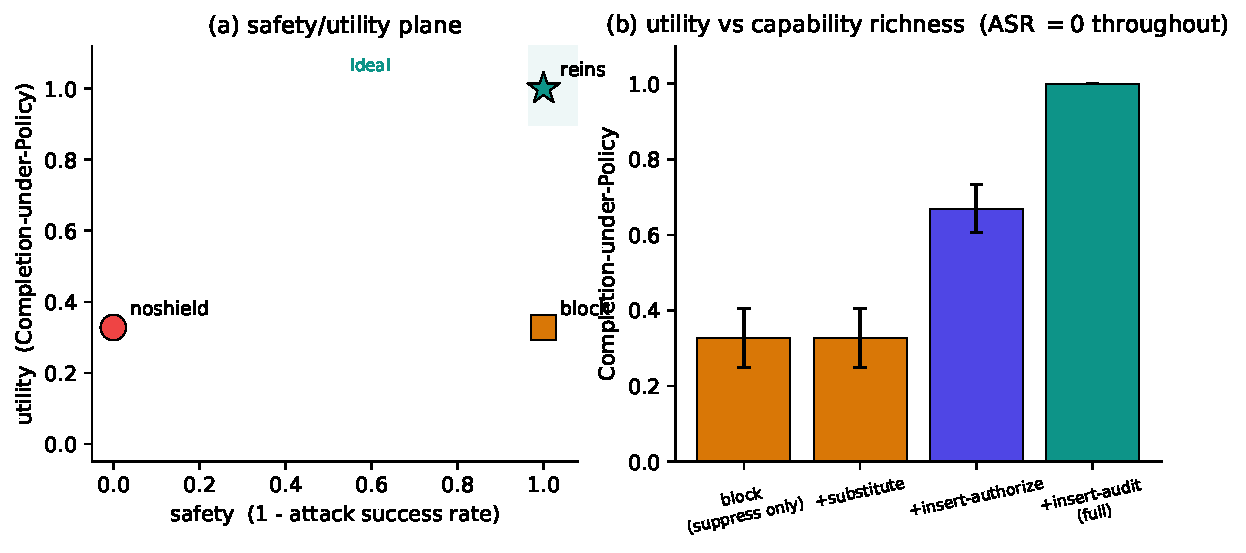
\includegraphics[width=0.98\linewidth]{figures/frontier.pdf}
\caption{E1: (a) the safety/utility plane, where REINS sits in the ideal corner,
matching blocking's safety with no-shield's utility; (b) CuP rises with
capability richness, all at ASR~$=0$.}
\label{fig:frontier}
\end{figure}

\begin{figure}[t]\centering
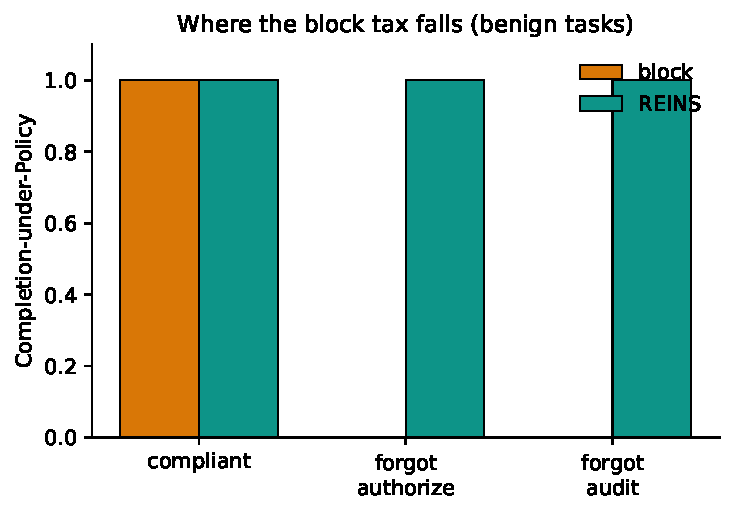
\includegraphics[width=0.6\linewidth]{figures/blocktax.pdf}
\caption{E1: the block tax falls on benign tasks that omit a prerequisite; REINS
repairs them by injection.}
\label{fig:blocktax}
\end{figure}

\subsection{E2: soundness and shieldability}
I fuzz $200$ random adversarial trajectories per seed. On a shieldable
deployment, $\soundFull$ of shielded sessions are sound with $\failFull$
enforcement failures, Theorem~\ref{thm:sound} in practice. A deployment the
static check flags as \emph{non}-shieldable (a required audit not insertable, no
escalation) does suffer failures ($\failBadNoEsc$ over the suite, soundness
$\soundBadNoEsc$); restoring the escalation channel returns soundness to
$\soundBadEsc$ via deferral, the trivial Schneider guarantee
(Figure~\ref{fig:minimality}, left). The static check predicts both, so the
trade-off is visible before deployment.

\subsection{E3: transparency and minimal intervention}
On already-compliant streams the shield's intervention rate is
$\interventCompliant$: it is the identity (Theorem~\ref{thm:transp}). Over
$\stepsChecked$ steps of an adversarial fuzz, every committed edit equals the
least-cost safe edit computed by a brute-force per-step oracle, a
certified-minimal rate of $\certMinRate$ (Proposition~\ref{prop:min}, and what the
certificate's minimality check re-derives). A branch-and-bound \emph{global}
optimiser on $\globalTraj$ short trajectories finds that the per-step optimum
coincides with the whole-trajectory optimum on $\globalAgree$ of them: high, but
\emph{not} $1$ (the largest myopic overspend was $\globalGap$ cost units). I
report this honestly rather than overclaim global optimality
(Figure~\ref{fig:minimality}).

\begin{figure}[t]\centering
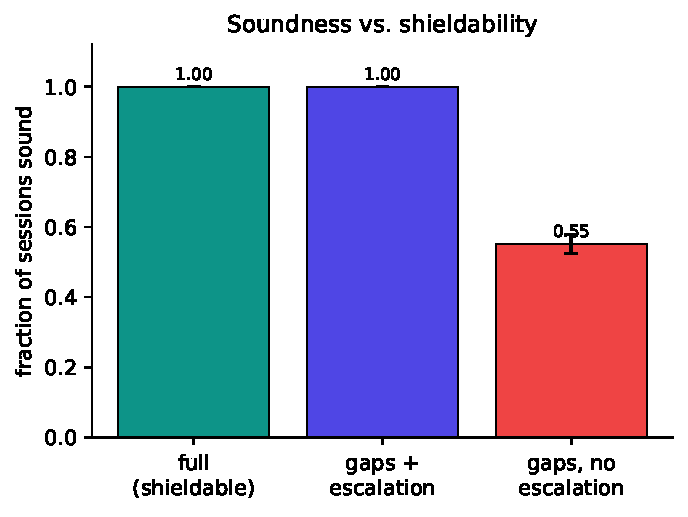
\includegraphics[width=0.49\linewidth]{figures/soundness.pdf}\hfill
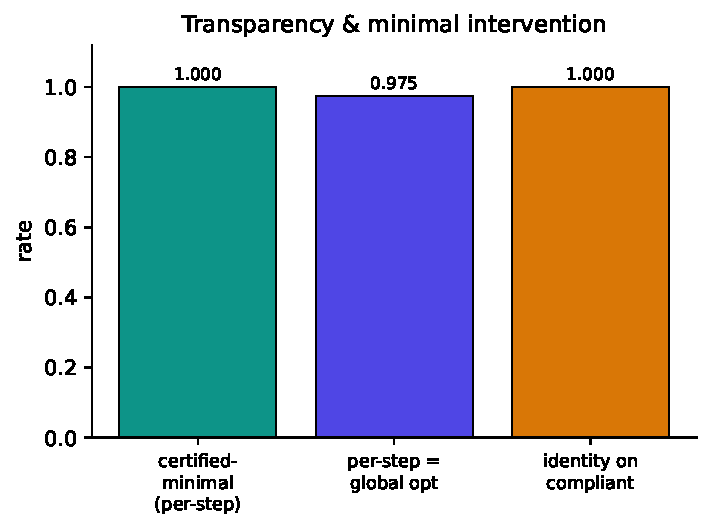
\includegraphics[width=0.49\linewidth]{figures/minimality.pdf}
\caption{E2 (left): soundness tracks shieldability. E3 (right): the shield is
identity on compliant streams, certifiably minimal per step, and matches the
global optimum on $\globalAgree$ of trajectories.}
\label{fig:minimality}
\end{figure}

\subsection{E4: the certificate}
I seal sessions and apply six structural tamper classes plus a key-less forgery:
all are detected ($\tamperRate$; Figure~\ref{fig:certificate}a). In
\emph{validly-signed} logs I then plant non-minimal records: rewriting a
substitute as a suppress (over-restriction) is caught at rate $\overCaught$, and
rewriting an intervention as an unguarded allow (under-restriction) is caught
$\underCaught/\underTrials$. The minimality re-verification flags both while
integrity stays intact. Verification re-runs the entire shield model-free in
$\verifyUs\,\mu$s for a $\verifyEntries$-entry session and is linear in entries
(Figure~\ref{fig:certificate}b).

\begin{figure}[t]\centering
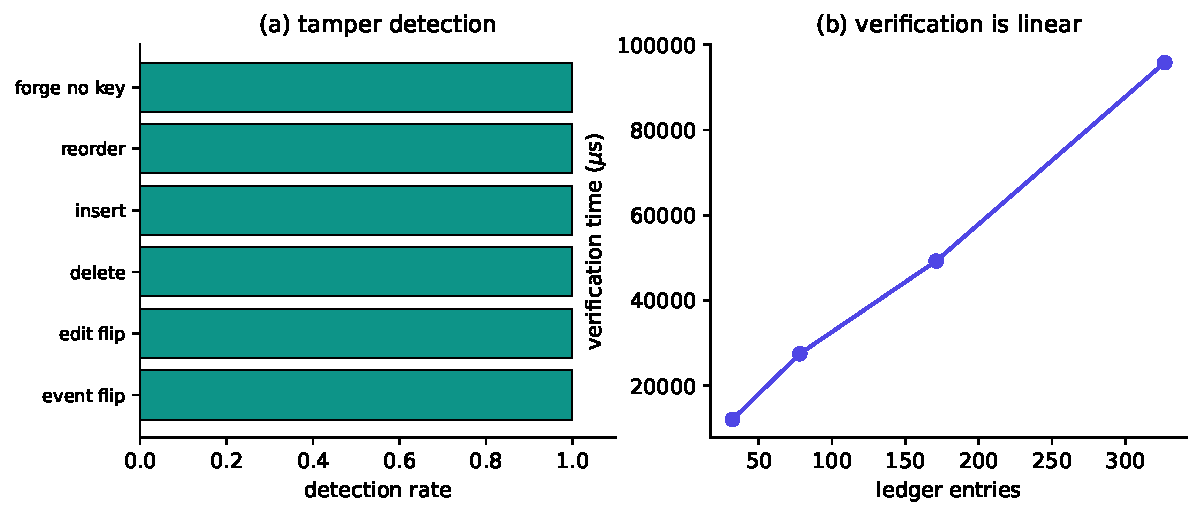
\includegraphics[width=0.98\linewidth]{figures/certificate.pdf}
\caption{E4: (a) every tamper class is detected; (b) model-free verification is
linear in ledger entries.}
\label{fig:certificate}
\end{figure}

\subsection{E5: systems}
A shield step costs $\shieldMed\,\mu$s median ($\shieldPnn\,\mu$s p99),
enumerating $\candMean$ candidates; monitor state is $\monMem$\,bytes and constant
in trajectory length (Proposition~\ref{prop:cost}); the ledger is
$\sim\ledgerBytes$\,bytes per entry. Latency grows sub-linearly with the number of
constraints (Figure~\ref{fig:systems}) and stays well under a millisecond: REINS
is as deployable inline as the monitors it enforces, on CPU.

\begin{figure}[t]\centering
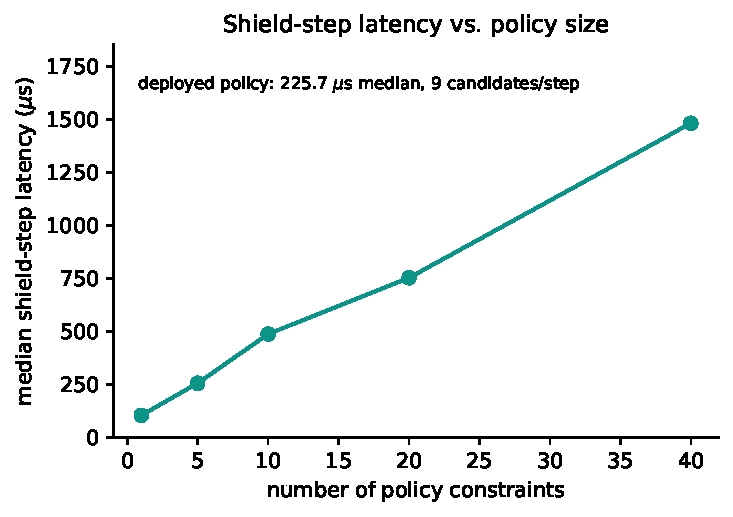
\includegraphics[width=0.6\linewidth]{figures/systems.pdf}
\caption{E5: shield-step latency vs.\ policy size; sub-millisecond on a CPU.}
\label{fig:systems}
\end{figure}

\subsection{E6: robustness and honest failure modes}
\label{sec:robust}
Three probes, two adversarial to my own claims (Figure~\ref{fig:robustness}).
\emph{First}, an adaptive exfiltration attacker is \emph{bounded}: REINS caps
executed external sends at the rate budget ($\le\exportBudget$) no matter how many
are attempted, bounding the damage rather than being fooled. \emph{Second},
REINS is only as strong as its declared capabilities: with the utility-preserving
edits removed its benign CuP collapses to the blocking level ($\ablNoIns$ vs
$\ablFull$), and \emph{without an escalation channel as well} even soundness
degrades ($\ablNoEscSound$), exactly the regime the static shieldability check
warns against. \emph{Third}, REINS guarantees safety with respect to the
\emph{declared} events, not un-modelled real-world effects: a mis-declared ``safe''
substitute is trusted, but it is recorded verbatim in the certificate
($100\%$ of substitutions are auditable), so the deployer's error is auditable
even though it is not prevented. I also note the per-step/global gap of E3 and
that the benchmark is synthetic.

\begin{figure}[t]\centering
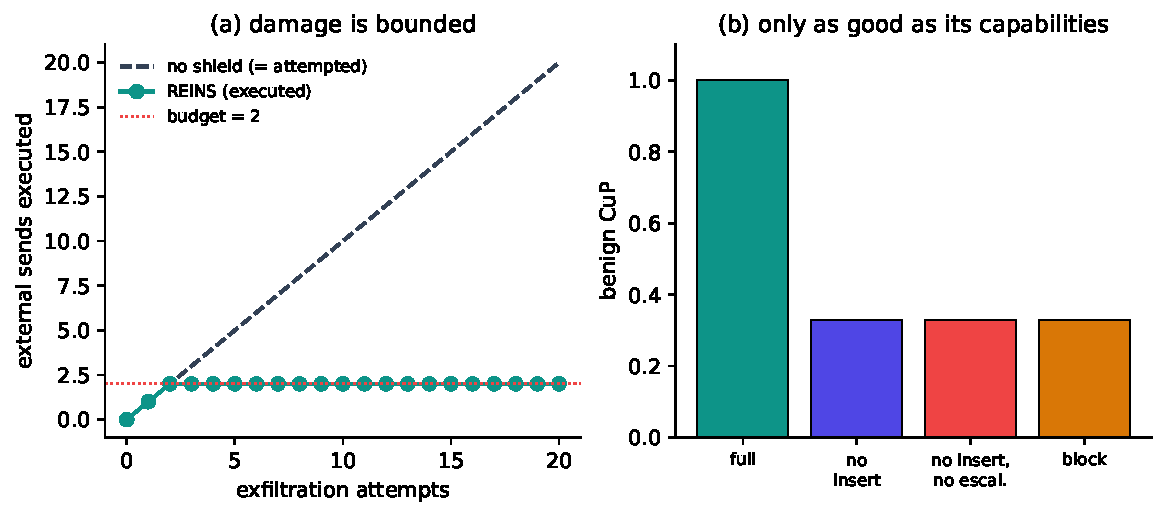
\includegraphics[width=0.98\linewidth]{figures/robustness.pdf}
\caption{E6: (a) the rate monitor bounds exfiltration damage; (b) REINS is only as
strong as its declared capabilities, so utility (and, without escalation, soundness)
degrades as they are removed.}
\label{fig:robustness}
\end{figure}

\subsection{E7: worked case studies}
Four canonical situations, with the human-readable receipts REINS emits:
a sensitive read missing its compliance log $\to$
\textsc{Insert}(\texttt{audit\_log}) at the deadline, read preserved;
a transfer missing authorisation $\to$ \textsc{Insert}(\texttt{authorize}),
transfer proceeds; a destructive \texttt{delete\_all} $\to$
\textsc{Substitute}(\texttt{archive}); a slow-roll over-budget send $\to$
\textsc{Suppress}. In each the blocking guardrail aborts the task; REINS keeps it
moving while staying in the safe language, and the certificate records exactly
what it did and why.

\section{Discussion}
REINS instantiates a \emph{model-free}, \emph{least-cost}, \emph{certifying} repair
shield, a combination the contemporary LLM-agent enforcers in
Table~\ref{tab:compare} do not jointly provide. It does not
need the model in the loop, so it shields closed and black-box agents on CPU; it
preserves task utility where blocking destroys it; and it produces an auditable
certificate that the agent was neither under- nor over-restricted, directly
serviceable for EU AI Act record-keeping and human-oversight obligations. It is
not a new enforcement theory: it stands on edit
automata~\citep{ligatti2005edit}, shield
synthesis~\citep{bloem2015shield,alshiekh2018safe}, optimal
enforcement~\citep{pandya2019optimal,gallay2021decentralized}, and certifying
algorithms~\citep{mcconnell2011certifying}, and its value is their specific
deployable, certifying conjunction for agents.

\paragraph{When to use REINS.} Where an agent must keep working under a declared
temporal policy and every intervention must be \emph{explained and certified}:
regulated deployments, on-device/edge agents, or a cheap auditable enforcement
layer in front of a heavier neural guardrail.

\section{Limitations and future work}
\label{sec:limits}
\begin{itemize}[leftmargin=1.4em,itemsep=1pt]
\item \textbf{Capability-bound.} REINS is only as strong as its declared
capabilities and substitution table; inadequate capabilities collapse it toward
blocking, and a mis-declared substitute is trusted (\S\ref{sec:robust}). The
static check surfaces the former; the certificate makes the latter auditable.
\item \textbf{Per-step, not global.} I prove and certify per-step minimality;
the per-step optimum matched the whole-trajectory optimum on $\globalAgree$ of
trajectories but not all. A bounded-lookahead planner is future work.
\item \textbf{Declared-policy coverage.} REINS enforces only constraints someone
wrote; mining bounded-LTL policies from agent logs~\citep{lemieux2015texada} is the
natural front-end.
\item \textbf{Synthetic benchmark.} The trajectories follow published taxonomies
but are not a live agent harness; an AgentDojo~\citep{debenedetti2024agentdojo}
and ST-WebAgentBench~\citep{levy2025stwebagentbench} evaluation, and a head-to-head
against AgentSpec and Agent-C, are future work.
\item \textbf{Symmetric authentication only.} The reference ledger is HMAC-based;
an Ed25519 signature over the Merkle root upgrades it to non-repudiation.
\end{itemize}

\section{Ethics and broader impact}
This work is defensive. The benchmark is synthetic and contains no personal data.
I disclose REINS's failure modes (\S\ref{sec:robust}) precisely so deployers do
not over-trust it: a shield that silently degrades to blocking, or trusts a wrong
substitute, is dangerous if mistaken for complete. The interpretable policy and
the certificate reveal the enforcement logic to an adversary; I judge the
auditability benefit to outweigh this, consistent with open-source security
practice.

\section{Reproducibility}
The repository contains the library, the unit-test suite, the seven experiments,
the figure and number scripts, and this paper's source. \texttt{python -m pytest}
runs the tests; \texttt{python experiments/run\_all.py} regenerates every
\texttt{results/*.json}; \texttt{python scripts/make\_figures.py} and
\texttt{paper\_numbers.py} rebuild the figures and the macro file; the host,
seeds and protocol are disclosed in \S\ref{sec:exp}.

\section{Conclusion}
A guardrail need not choose between seeing an unsafe action and stopping the task.
REINS shows that a runtime shield can keep an LLM agent inside an interpretable
temporal policy by the \emph{least-cost enactable edit} (injecting a missing
authorisation or audit, downgrading a dangerous tool, suppressing, or deferring),
\emph{model-free on CPU}, and seal each intervention into a certificate an auditor
re-checks without the model, proving the agent was neither under- nor
over-restricted. It dominates the safety/utility frontier over blocking at
identical safety. Standing openly on the edit-automata and shielding lineage, its
contribution is their deployable, certifying instantiation for agents, a concrete
step toward guardrails that are not only effective but \emph{accountable}.

\bibliography{references}
\end{document}
